\documentclass[letterpaper,12pt]{article}
\usepackage{amsmath}  % improve math presentation
\usepackage{graphicx} % takes care of graphic including machinery
\usepackage{mathrsfs}


\usepackage[final]{hyperref} % adds hyper links inside the generated pdf file
\hypersetup{
	colorlinks=true,       % false: boxed links; true: colored links
	linkcolor=blue,        % color of internal links
	citecolor=blue,        % color of links to bibliography
	filecolor=magenta,     % color of file links
	urlcolor=blue         
}

\title{Tenth Assignment for Computational Physics}
\date{\today}
\author{Xinyu Liu}

\begin{document}
\maketitle
\tableofcontents

\section{Problem 1: Using Crank-Nicolson method to solve Schrodinger equation}

The associated code is in the 10-1.py.

In the code, we first explicitly realized the Crank-Nicolson which is essentially a forward-time method but it holds the numerical stability. In essence, we need to solve such a equation to know how our solution propagate with time:

\begin{align}
    \psi(x, t+h)-h \frac{\mathrm{i} \hbar}{4 m a^2} & {[\psi(x+a, t+h)+\psi(x-a, t+h)-2 \psi(x, t+h)] } \\
    & =\psi(x, t)+h \frac{\mathrm{i} \hbar}{4 m a^2}[\psi(x+a, t)+\psi(x-a, t)-2 \psi(x, t)]
\end{align}

This can be simply written down as:



Where A and B are symmetrical tridiagonal matrice:


\begin{equation}
    \mathbf{A}=\left(\begin{array}{llllll}
        a_1 & a_2 & & & \\
        a_2 & a_1 & a_2 & & \\
        & a_2 & a_1 & & \\
        & & a_2 & & \\
        & & & a_1 & \\
        & & & & \ddots
        \end{array}\right), \quad \mathbf{B}=\left(\begin{array}{lllll}
        b_1 & b_2 & & & \\
        b_2 & b_1 & b_2 & & \\
        & b_2 & b_1 & b_2 & \\
        & & b_2 & b_1 & \\
        & & & & \ddots
    \end{array}\right)
\end{equation}

This mean that, the propagation of wave function is:

\begin{equation}
    \psi(t+h)= \mathbf{A^{-1}}  \mathbf{B} \psi(t)
\end{equation}

After setting all the parameters as instructed. We start to numerically solve the evolution of wave function under schrodinger equation. What's worth noting here is that, although in the problem it propose some faster method to invert a tridiagonal matrice, I've found that it's not slow to do standard inversion for matrice $\mathbf(A)$. First, the matrice inversion only need to be done once. Also, the matrice calculation in numpy is pretty fast. We found that by this stupid matrice multiplication method we can evolution of 1000 steps in around 1s if we discretize the waveequation in 1000 spots(as instructed).

Then I use the FuncAnimation method in matplotlib to create an animation of the evolution of the wave equation. Since this result is a bit hard to show in this pdf, I suggest that you could go to the code and execute it by yourself. Here I just provide with some screenshot along with description of the evolution.
\newpage


Initially, the wavefunction is some kind of well localized propagating wavepacket. As time evolves, the localized wavepacket become more and more dispersed and also the center of the wavepacket(or to say the expectation position of the particle) is bounced back and force between walls. It goes as follows:

\begin{table}[!h]
    \centering
    \caption{The evolution of wave function: picture 1}
    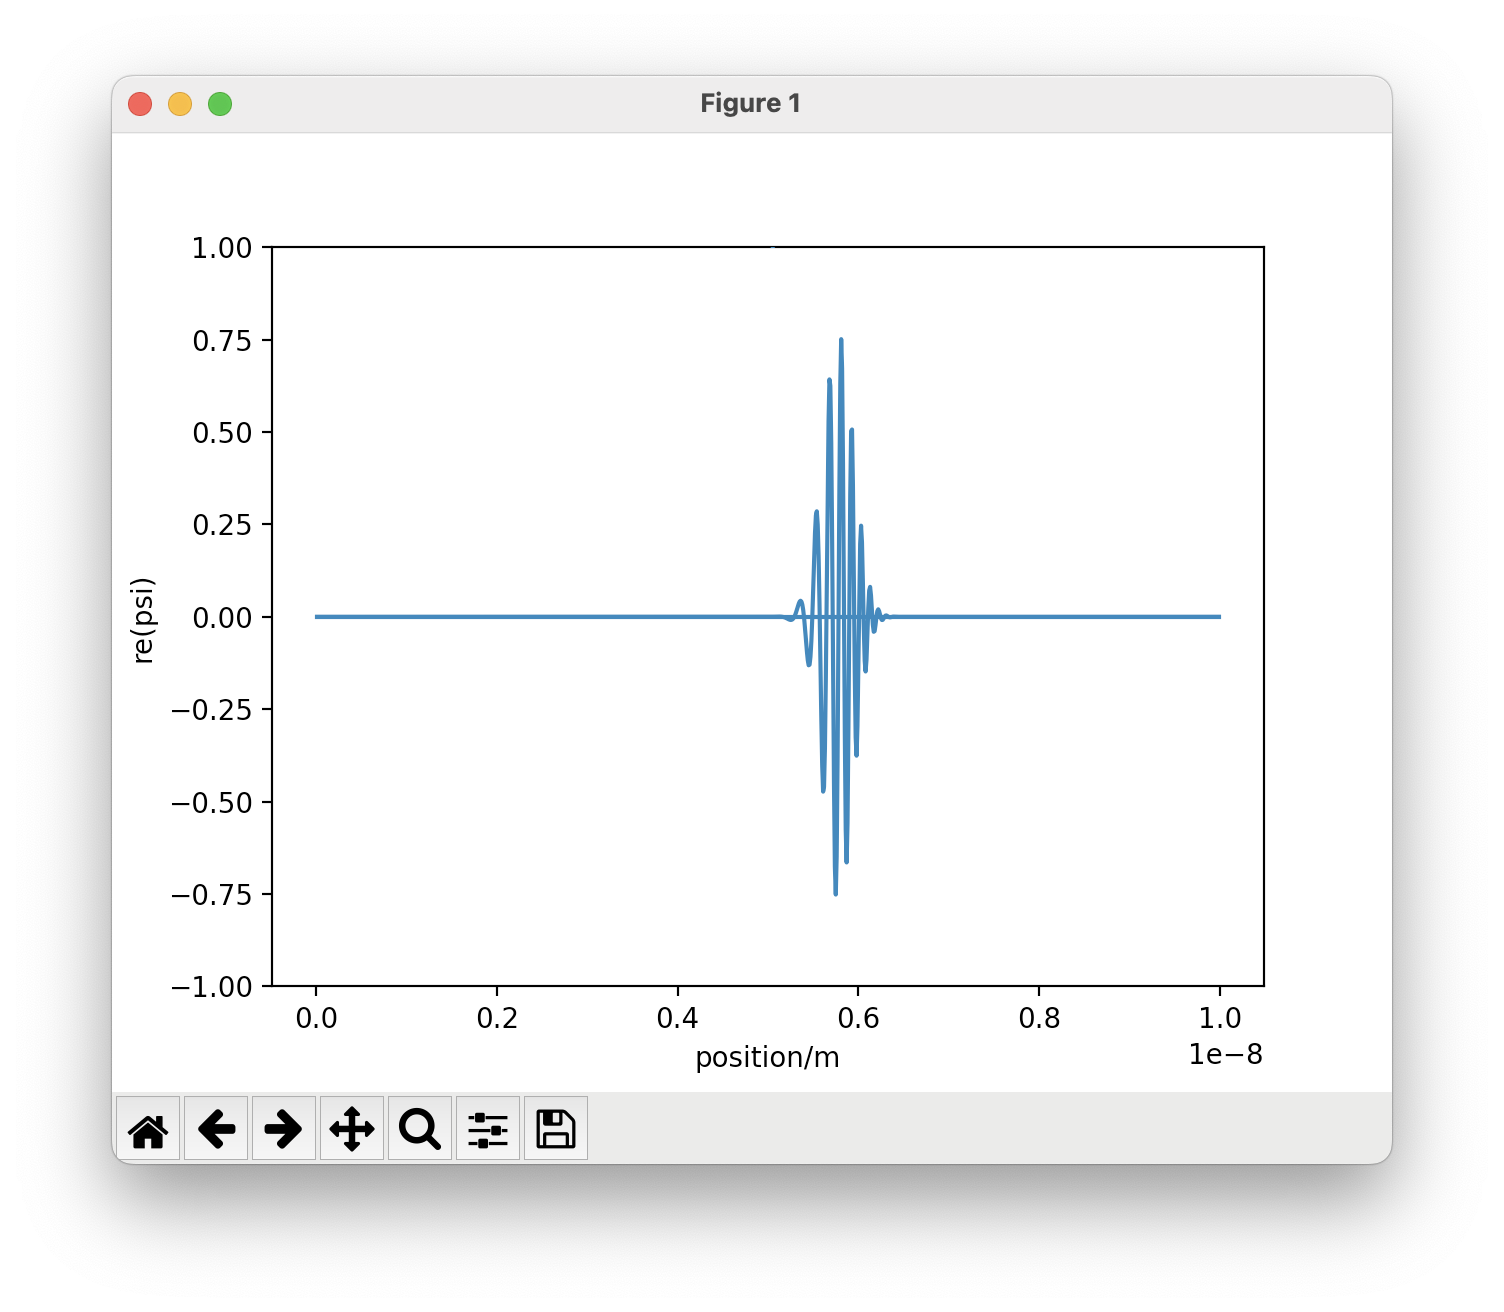
\includegraphics[width=13cm]{1}
\end{table}%
\newpage



\begin{table}[!h]
    \centering
    \caption{The evolution of wave function: picture 2}
    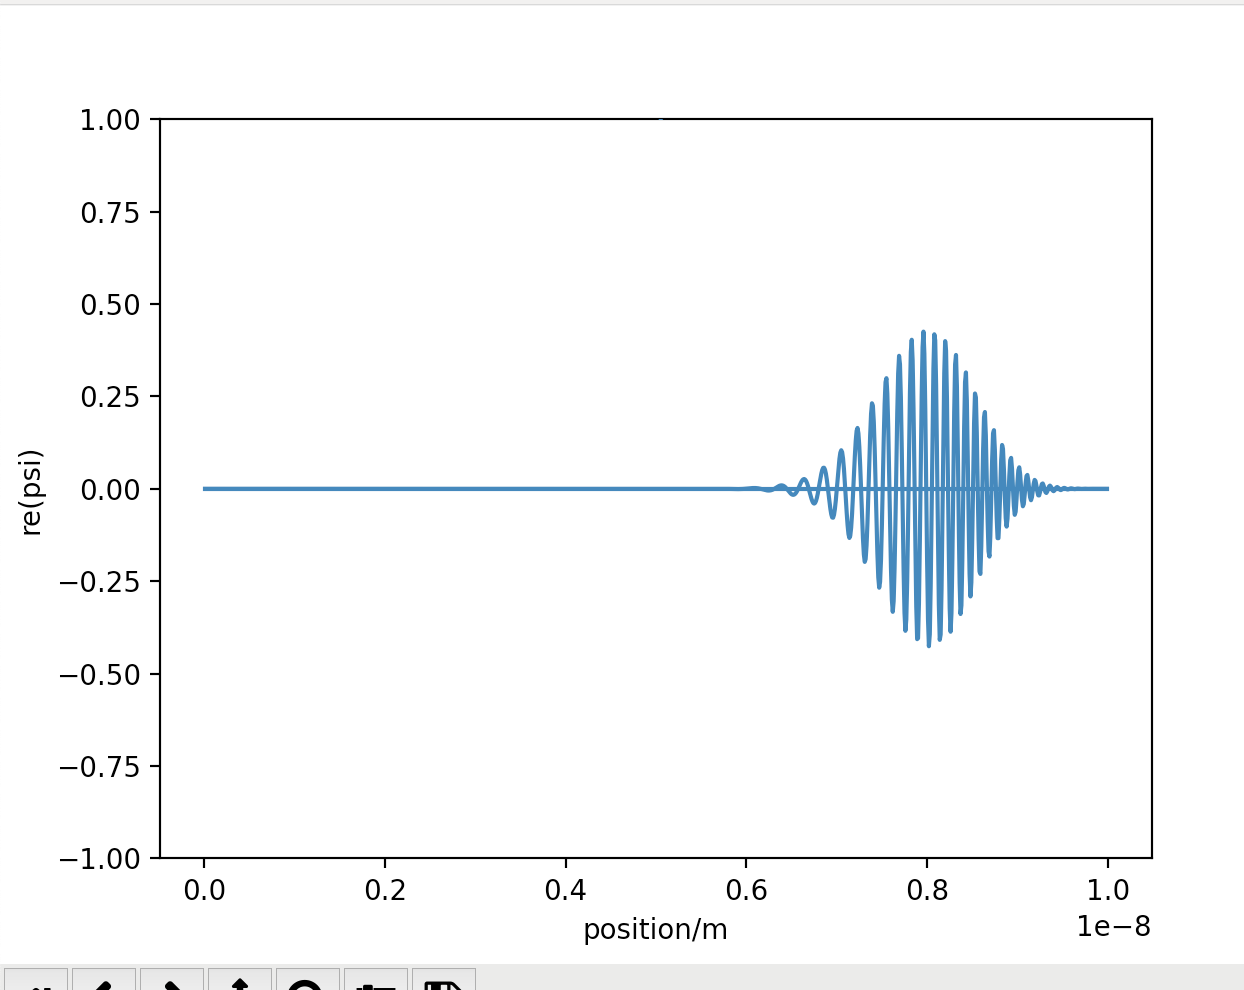
\includegraphics[width=10cm]{2}
\end{table}%

\begin{table}[!h]
    \centering
    \caption{The evolution of wave function: picture 3}
    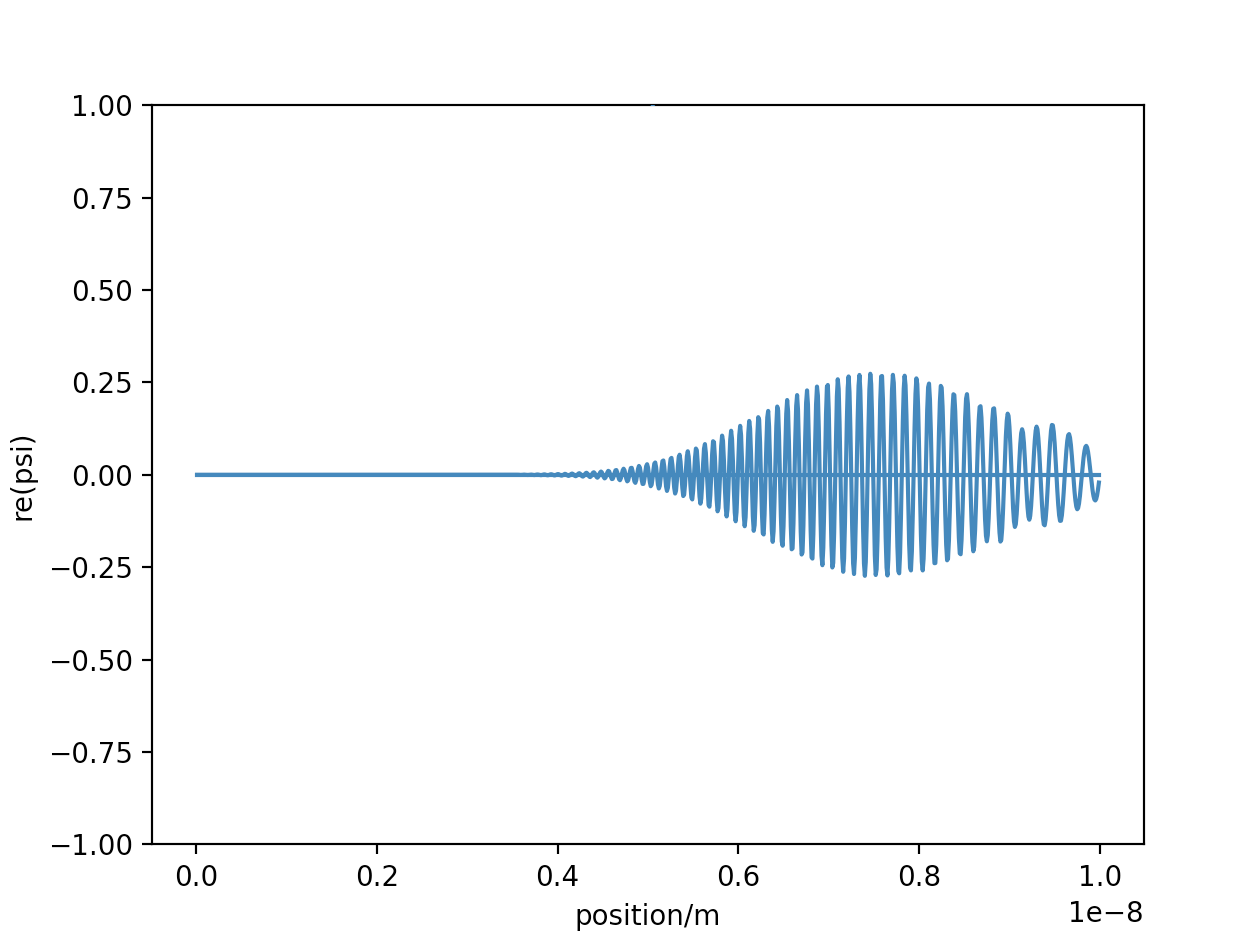
\includegraphics[width=10cm]{3}
\end{table}%
\newpage

\begin{table}[!h]
    \centering
    \caption{The evolution of wave function: picture 4}
    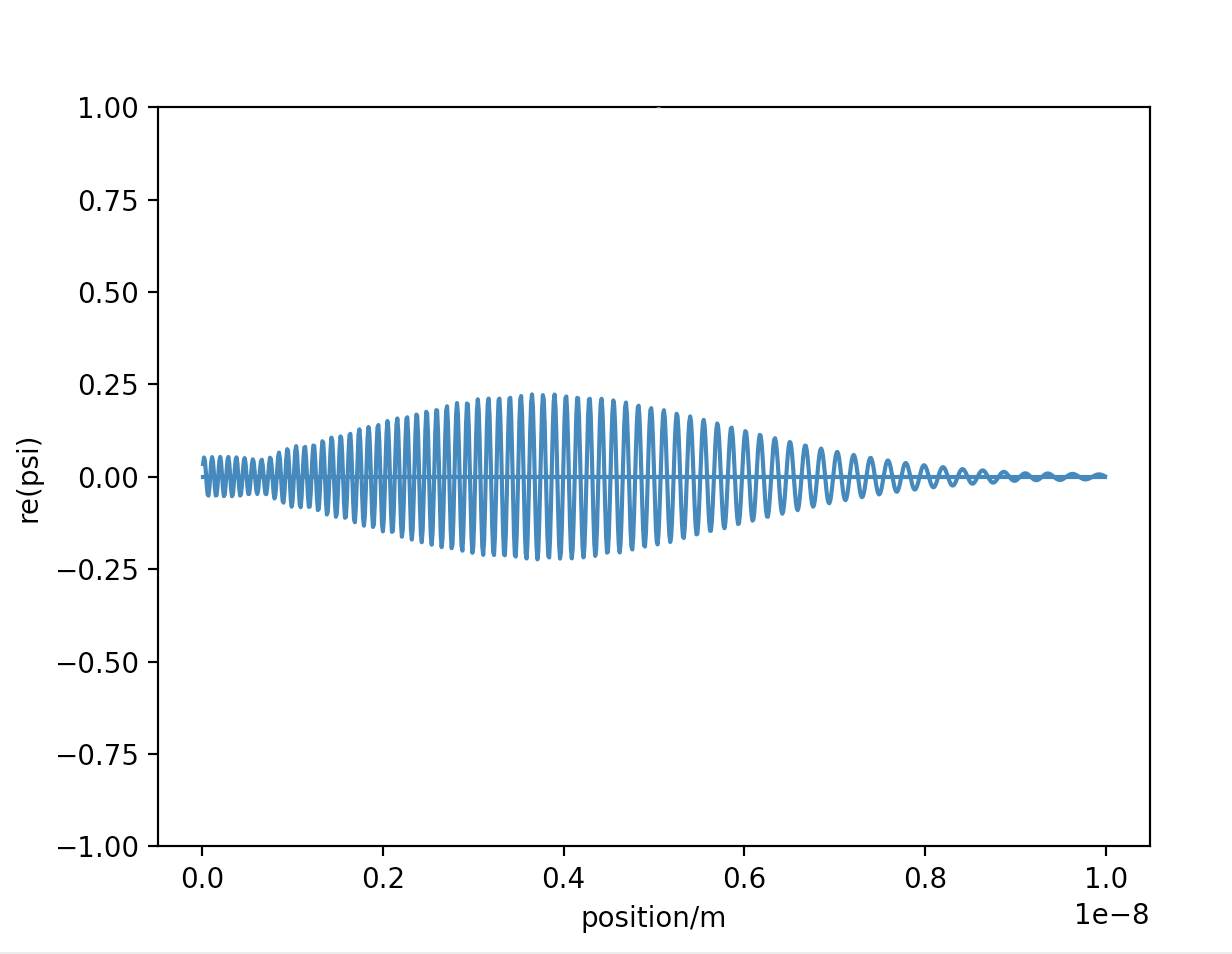
\includegraphics[width=9cm]{4}
\end{table}%

Finally, when it evolves for very long time, the wavepacket is so large(which is no longer important in comparison to the size of the potential well) and the particle somehow become more evenly distributed in the whole potential well.

\begin{table}[!h]
    \centering
    \caption{The evolution of wave function after long time}
    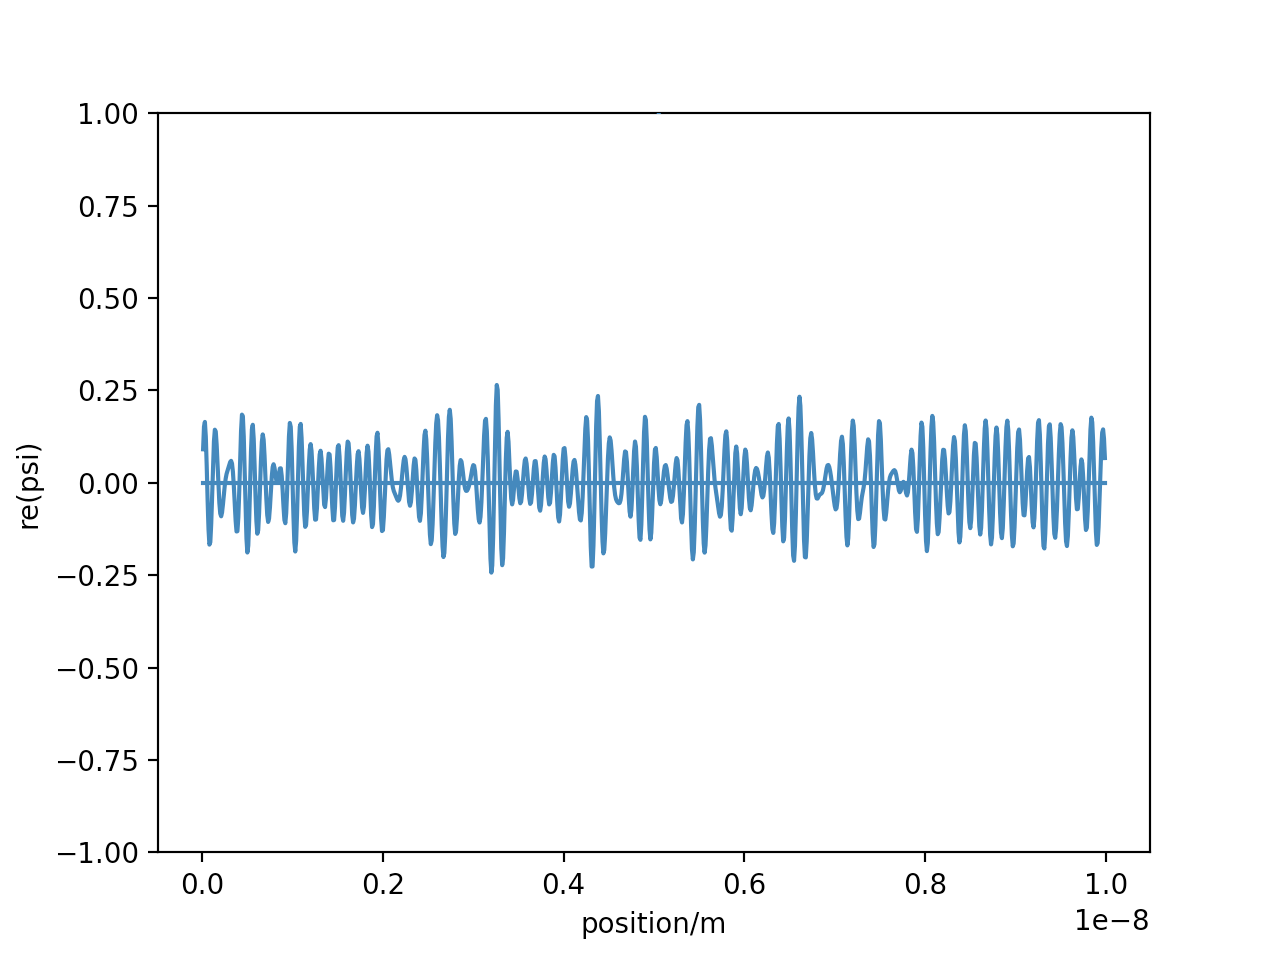
\includegraphics[width=9cm]{6}
\end{table}



\section{Problem 2: Using spectral method to solve Schrodinger equation}

The code associated with this part is 10-2.py

The physical situation and simulation parameter of this part is the same as previous problem. The only difference is that now we apply a different method to calculate the evolution of the system. The spectrum method applied in this part is related to time-independent schrodinger equation method in physics. We first solve the eigenmode of the system and project our initial state to those eigenmode. Since the evolution of the eigenmode is very simple, we can know the wavefunction at any future time.

Since for a free field schrodinger equation $-\frac{\hbar^2}{2 M} \frac{\partial^2 \psi}{\partial x^2}=\mathrm{i} \hbar \frac{\partial \psi}{\partial t}$ in a infinite deep potential well, the eigenmode is actually just sine waves, which evolves as:

\begin{equation}
    \psi_k(x, t)=\sin \left(\frac{\pi k x}{L}\right) \mathrm{e}^{\mathrm{i} E t / \hbar}
\end{equation}

This makes the projection to eigenmode pretty easy, which as a result is simply fourier transform. So in the code, we first use dst to do fast sine wave decomposition to get the fourier coefficients. This dst method can be imported from scipy module. The wave function at any time can be expressed by:

\begin{equation}
    \psi\left(x_n, t\right)=\frac{1}{N} \sum_{k=1}^{N-1} b_k \sin \left(\frac{\pi k n}{N}\right) \exp \left(\mathrm{i} \frac{\pi^2 \hbar k^2}{2 M L^2} t\right)
\end{equation}

By putting $b_k=\alpha_k+\mathrm{i} \eta_k$ we can get the real part of the wavefunction at anytime t:

\begin{equation}
    \operatorname{Re} \psi\left(x_n, t\right)=\frac{1}{N} \sum_{k=1}^{N-1}\left[\alpha_k \cos \left(\frac{\pi^2 \hbar k^2}{2 M L^2} t\right)-\eta_k \sin \left(\frac{\pi^2 \hbar k^2}{2 M L^2} t\right)\right] \sin \left(\frac{\pi k n}{N}\right)
\end{equation}

We can then plot the wavefunction and create an animation similarly with FuncAnimation method. \textbf{This animation and description part is exactly the same as the previous problem so I'll neglect it in this report}. We simply present the wavefunction of the particle at time $t = 10^{-16}s$:

\begin{table}[!h]
    \centering
    \caption{The wavefunction of particle at $t = 10^{-16}s$}
    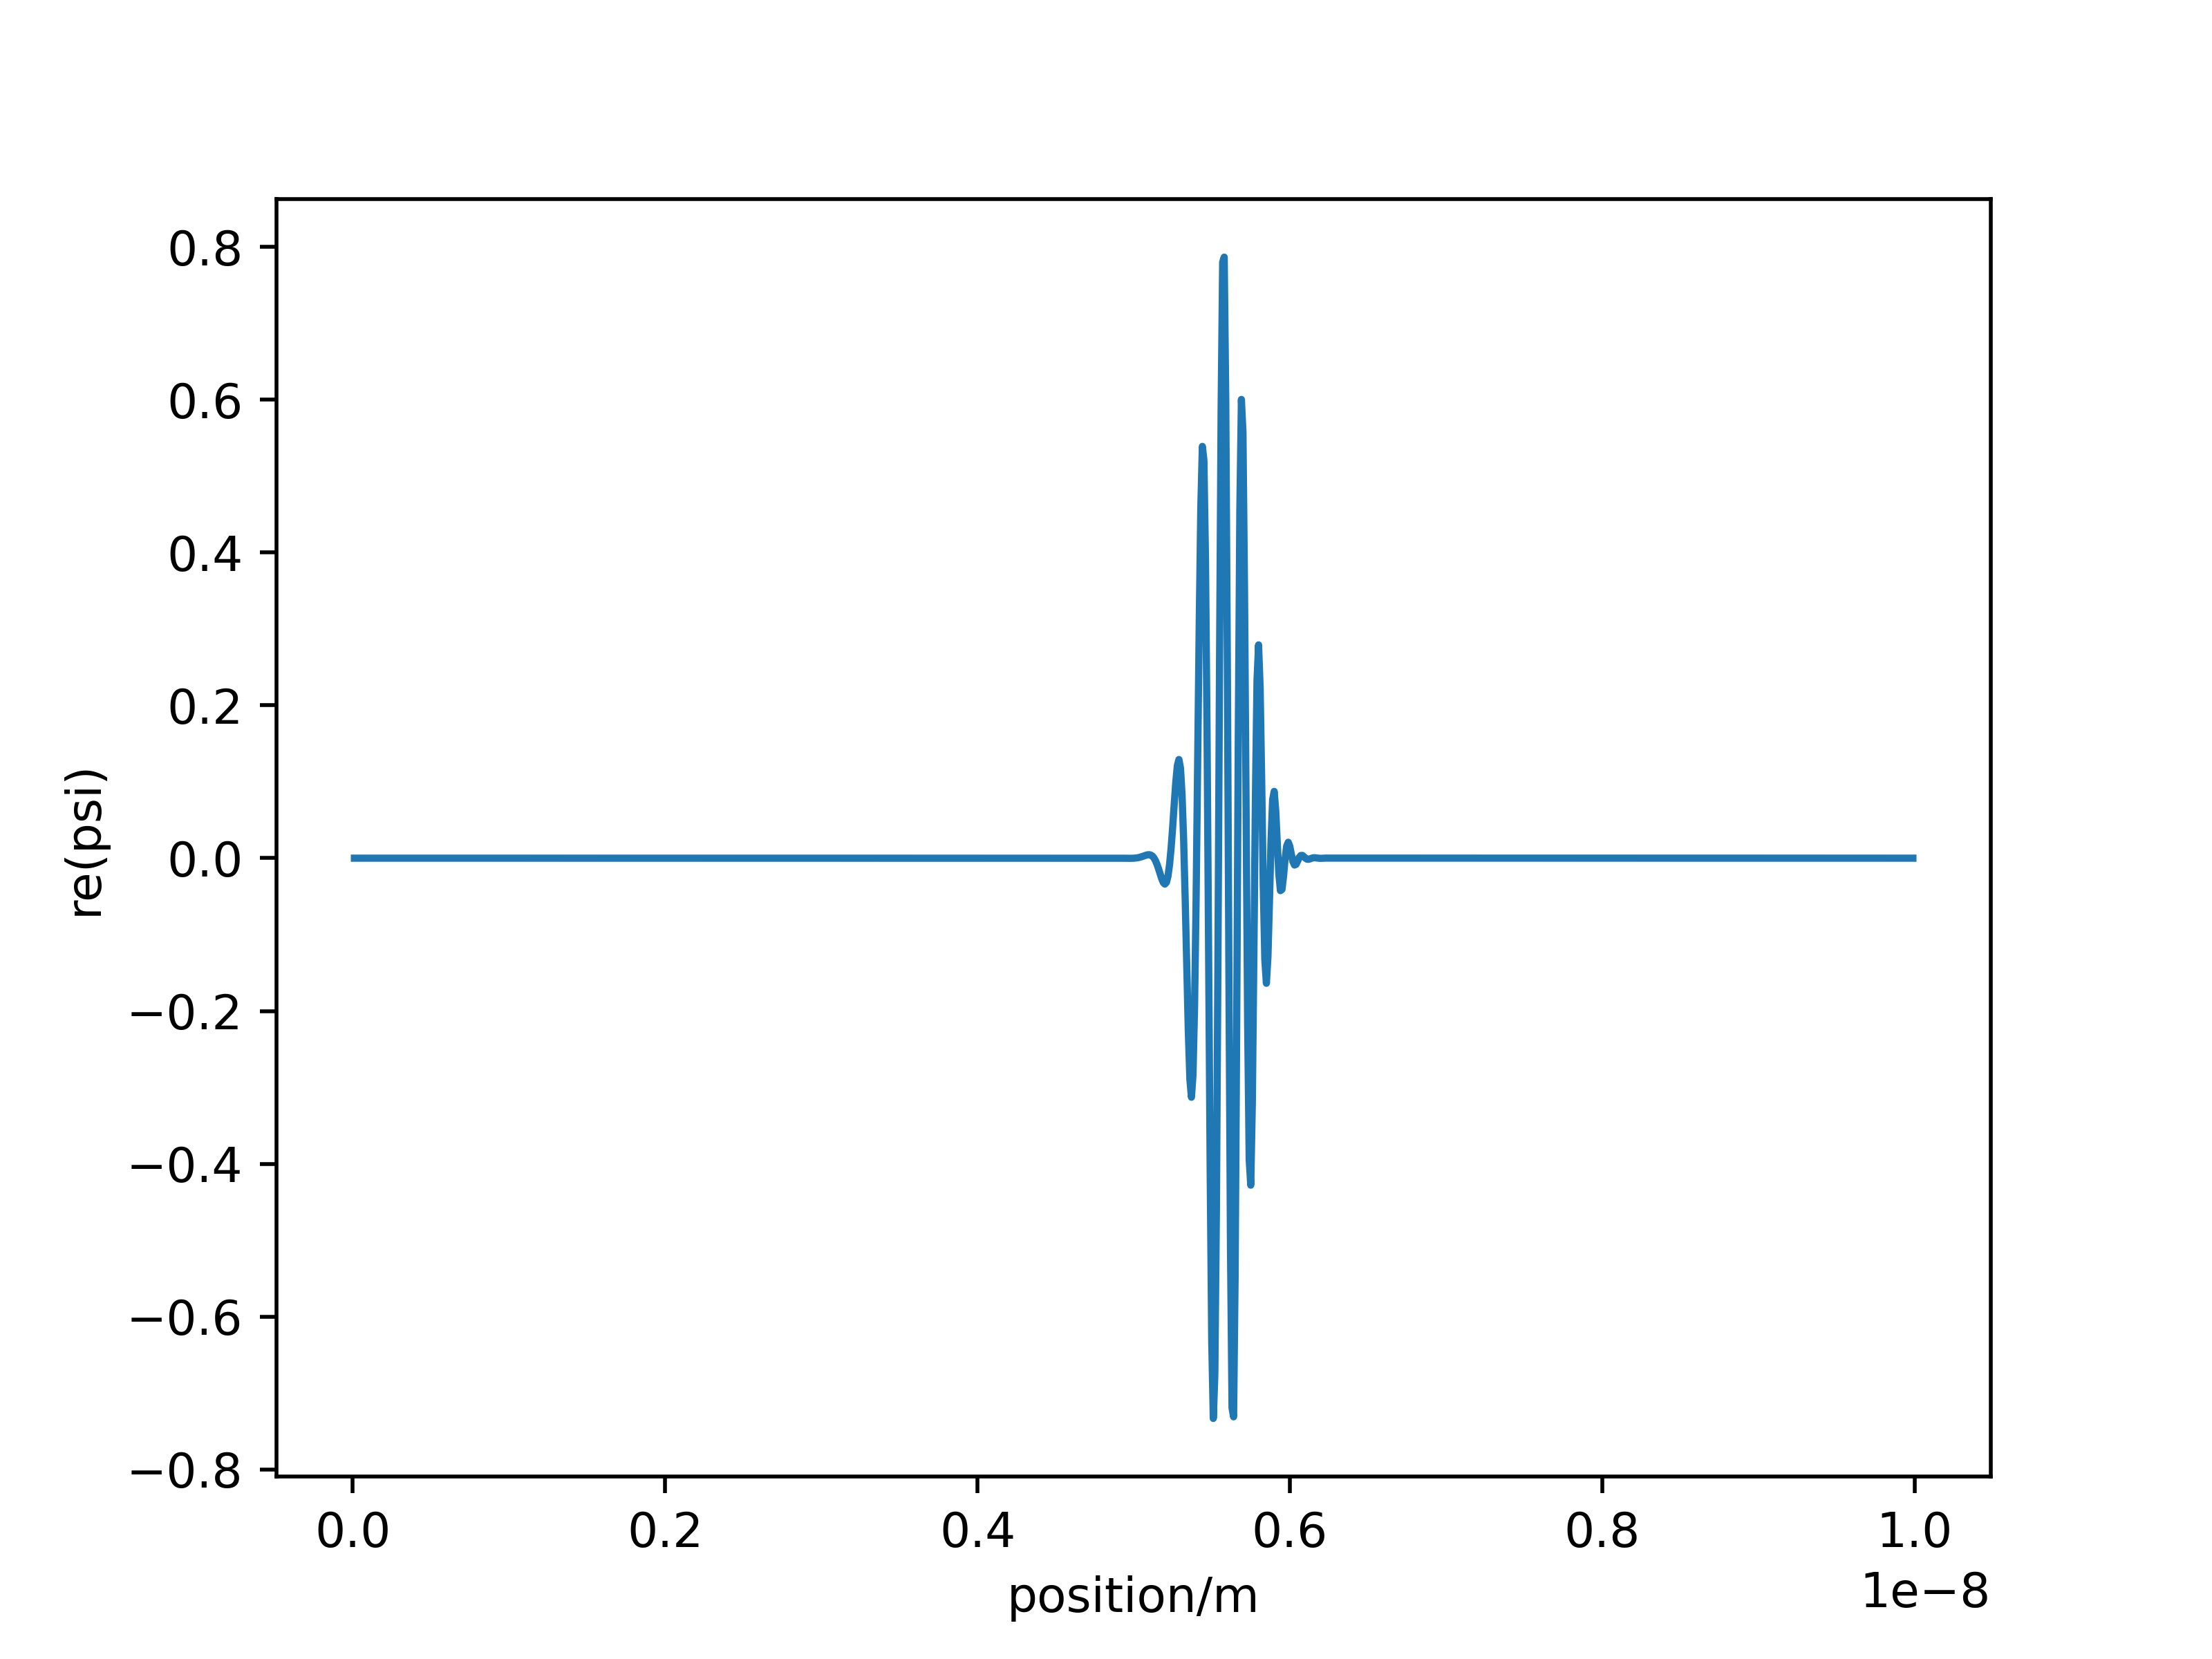
\includegraphics[width=13cm]{7.png}
\end{table}%


\end{document}